%!TeX root=../../main.tex
\chapter{Proposed Solution}                                 \label{ch:solution}

In this thesis, we aim to create an algorithm that, once running on one of the control plane nodes of a \acrshort{k8s} cluster, continuously watches the state of that cluster and detects any conflicts between the cloud and cluster layer. To achieve this we capture the six types of events that can influence the connection between containers in the cluster layer as seen in \autoref{tab:events}. When one of these events is captured an automatic conflict detection should be triggered and the algorithm must report on all possible conflicts between the cloud and cluster layer. Additionally all pods and \acrshort{np}s affected by an event must get checked for redundancy. e.g. after the deletion of the last pod that matches a \acrshort{np} label selector it must report that that policy has become redundant. Lastly, it should be noted that changes in the cloud layer can influence connections as well (e.g. security groups being created) but this is outside the scope of this thesis.
\\[10pt]
\begin{table}[htbp]
  \centering
  \begin{tabular}{|c|c|}
    \hline
    pod & \acrshort{np} \\
    \hline
    create & create \\
    delete & delete \\
    update & update \\
    \hline
  \end{tabular}
  \caption{watcher events}
  \label{tab:events}

\end{table}

In order to work incrementally we want to store all necessary information about the current state of the cluster. With this information, we can look directly at the relevant containers and \acrshort{np}s for each event and reduce the computation time. For example, there is no need to check containers that are not affected by a newly created network policy. We call this the incremental approach since it incrementally updates the stored cluster state with each event. As a bonus, we added a simple startup detection method that can detect conflicts upon the startup of the algorithm. periodically running this startup detection could serve as an alternative in case a continuously running algorithm would prove unviable in any way.  
\\[10pt]

We will only monitor a single namespace when executing the algorithm, which can be specified as an argument. Since the main purpose of namespaces is to isolate groups of resources within the cluster there should not be any communication between namespaces anyway which means conflicts can not exist \cite{namespace}. If required multiple instances of the algorithm can be run for different namespaces. We would also like to note that we will deploy only one container per pod in our algorithm and that therefore the terms pod and container might frequently be used as synonyms in the case of variables.
\\[10pt]

In the rest of this chapter, we will describe our solution, implemented in Python, that meets all the requirements and solves the problem of conflict detection between cloud and cluster layers. The implementation is based on a \acrshort{k8s} cluster with nodes deployed on an OpenStack installation. \autoref{fig:algorithm} demonstrates how the algorithm is split up into separate parts, which correlates directly to different Python files with the corresponding names and functionalities. We briefly summarize these functionalities for each component of the algorithm before describing them more in-depth:
\begin{itemize}
    \renewcommand{\labelitemi}{\scriptsize$\blacksquare$}
    \item \textit{Watcher:} The watcher initializes the other components and leverages the Python \acrshort{k8s} library to continuously monitor for each of the six events described in \autoref{tab:events}, which it will forward to the analyzer.
    \item \textit{Analyzer:} The analyzer orchestrates the handling of events passed by the watcher. First, these events must be forwarded to the parser to be turned into usable objects. Afterwards, the analyzer calls the \acrshort{kic} to update the reachability matrix and cluster state and the \acrshort{sgic} to look at this updated reachability matrix for conflicts.
    \item \textit{Parser:} The parser turns the event data from the watcher into objects that can be used by the Analyzer. Since its functionality is straightforward this component will not be described in depth in this chapter.
    \item \textit{\acrfull{kic}:} The \acrshort{kic} handles the incremental update of the reachability matrix and stores all information about the cluster state.
    \item \textit{\acrfull{sgic}:} The \acrshort{sgic} generates a randomised set of security groups and corresponding rules and binds them to nodes upon startup. Additionally, it performs conflict detection between the cluster and cloud layer.
    \item  \textit{Model}: The model defines data structures to be used within the other components. These data structures are often created by the parser out of event data, such as Container, Policy and Reachabilitymatrix objects. Finally, it leverages the Kano generation method to create a reachability matrix upon startup which offers the base matrix which we will update incrementally with each captured event.
    \item  \textit{LabelTree}: A labelTree is a custom tree-like data structure used to store \acrshort{np}s by their selector labels, for quick retrieval by the \acrshort{kic} later on.
\end{itemize}
\begin{figure}[htbp]
  \centering
  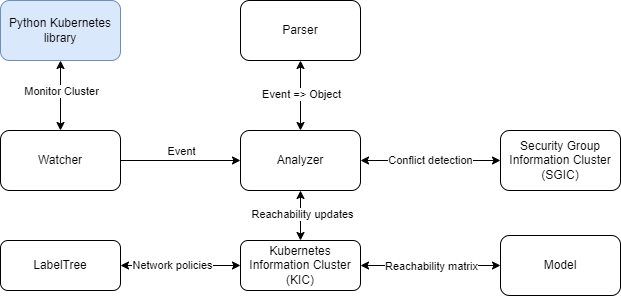
\includegraphics[width=0.8\textwidth]{images/algo-components.png}
  \caption{Algorithm structure}
  \label{fig:algorithm}
\end{figure}



% ==============================================
\section{Model} \label{impl:model} There are many data structures used in the algorithm, most of which are stored in the model file. To ensure a good understanding of these underlying structures in the other components we will first describe the ones that occur most often: the Policy, Container, Store and ReachabilityMatrix.
\\[10pt]

\textbf{Policy:} The Policy structure stores multiple variables which often are specific data structures on their own. We will not describe each of these sub-structures in-depth, but instead, briefly explain the most important variables:
\begin{itemize}
    \renewcommand{\labelitemi}{\scriptsize$\blacksquare$}
    \item \textit{name:} Stores the name of the policy. Although they are not enforced to be unique in the algorithm they will be in practice, since all objects in the same namespace must have unique names. 
    \item \textit{selector:} This data structure stores the labels which select the grouping of pods to which the policy applies.
    \item \textit{allow:} This data structure stores the labels that select the ingress sources or egress destinations.
    \item \textit{direction:} The direction is a boolean that indicates whether it is an ingress (True) or egress (False) policy.
    \item \textit{id:} The id is the identifier for the policy. The usage of the id field as the identifier is preferred above the usage of the name since it can be chosen and changed within the algorithm. The name on the other hand is defined by \acrshort{k8s} and can only be changed if the policy is removed and added under the new name.
\end{itemize}
Furthermore, the policy stores variables such as port and CIDR to provide further details that might be required for future work.
\\[10pt]

\textbf{Container:} The container has some overlap in variable names and usage with the Policy data structure, such as id and name. additionally, it stores a list of labels applied to the container, a string variable called nodeName for the node on which the container is deployed, and a matrix\_id. This last integer variable indicates which position in the kanomatrix this container corresponds to. Since the kanomatrix will change in size when containers get removed or added, this variable will often change throughout the algorithm's handling of events.
\\[10pt]

\textbf{Store:} The store is a custom structure that is based on a dict, which is the Python equivalent of a hash table. It takes two integers, which we will call the key-duo, which get combined as a tuple to serve as a key in the dict. The value related to this custom tuple key is a list that can store objects depending on the need. The data structure offers functions to retrieve the list coupled to a key-duo, add an item to the list coupled to a key-duo, remove a specific value within a specific key-duo's list, and remove the entire entry for a specific key-duo out of the dict. This data structure is used within the ReachabilityMatrix data structure to store the policies responsible for a connection between two containers. An example of a Store can be found in the next section describing the reachablityMatrix structure.
\\[10pt]

\textbf{ReachabilityMatrix:} The reachabilityMatrix data structure stores multiple variables, which all get values assigned when calling its most important function: $build\_matrix$. This function takes a list of containers and policies and generates the corresponding reachability matrix according to Kano's algorithm \cite{kano}. the generated matrix will then be used as a base that we will incrementally update for further events. During the creation of this matrix, many useful results get stored in variables for later usage which we will briefly describe:

\begin{itemize}
    \renewcommand{\labelitemi}{\scriptsize$\blacksquare$}
    \item \textit{dict\_pods:} This dict stores the containers (which all get deployed in seperate pods, hence the name) as values, with an incrementing list of numbers as keys. This variable ensures that the pods will be set in the same order when incrementally updating the matrix, thus keeping the unaffected rows and columns in the same position.
     \item \textit{dict\_pols:} Similar to dict\_pods but for network policies
     \item \textit{label\_map:} This is the hashmap of container labels as described in the Kano prefiltration algorithm in section \ref{kano:prefiltration}. 
     \item \textit{resp\_policies:} The resp\_policies is a Store object that stores the responsible \acrshort{np}s for each container connection. The key-duo will represent the from- and to-container of the connection respectively, while the values in the corresponding list are a set of 2 values. The first value of this set is always the ingress rule, while the second is the corresponding egress rule.
     \item \textit{matrix:} The result of the $build\_matrix$ function is stored in this variable: the reachability matrix created with the given containers and policies, stored as a list of bit arrays.
\end{itemize}

\autoref{fig:store} shows an example of a reachabilitymatrix and some corresponding variables. This could be the result of running the  $build\_matrix$ function given a list of 3 containers ($a$, $b$ and $c$) and a list of 6 policies ($u$, $v$, $w$, $x$, $ y$, $z$). We can see that three container connections are allowed by the given network policies, indicated as a 1 in the matrix. the resp\_pols Store object thus stores 3 key-duos in its dict, one for each connection. The connection between containers 1 and 3 is enabled by two sets of network policies: (1, 5) and (1,4) where the first policy in these duos is an ingress rule and the second an egress rule. When leveraging the dict\_pols and dict\_pods variables we can thus give the following statement:
\\[10pt] 
\textit{Container $a$ can send messages to container $c$, and this connection is allowed both by the combination of ingress rule $u$ and egress rule $y$ and the combination of ingress rule $u$ and egress rule $x$}.
\\[10pt]
Note that this also means there are redundant policies. We can remove policy $z$ since it is not used, and even policy $x$ or policy $y$ since one can replace the usage of the other.
\begin{figure}[H]
  \centering
  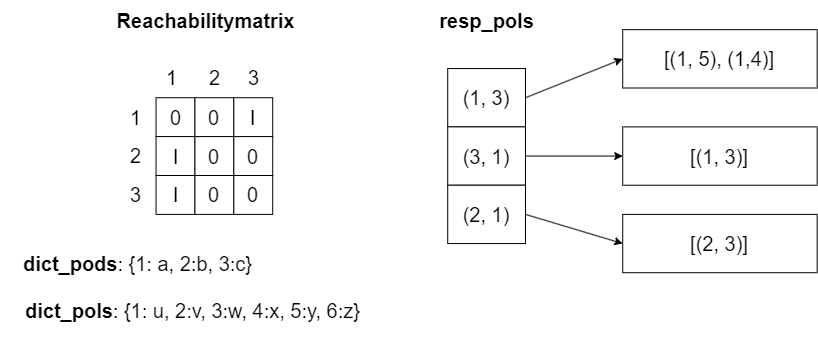
\includegraphics[width=0.8\textwidth]{images/store.png}
  \caption{Example of a reachabilitymatrix and some corresponding variables}
  \label{fig:store}
\end{figure}


% ==============================================
\section{Watcher} \label{impl:watcher} Execution of the algorithm starts by calling the main method of the watcher, which will then initialise all the other required components. The following flags and arguments are available when calling the watcher file:
\begin{itemize}
    \renewcommand{\labelitemi}{\scriptsize$\blacksquare$}
    \item \textbf{namespace:} The namespace in which the algorithm will look for conflicts (\textbf{required}).
    \item \textbf{verbose:} If the verbose flag is set, either by using -v or --verbose, the updated reachability matrix and corresponding container IDs will be printed after each event (\textbf{optional}). 
    \item \textbf{debug:} If the debug flag is set, either by using -d or --debug, all data structures will be printed out to provide more information about changes in the stored cluster state (\textbf{optional}).
    \item \textbf{startup:} If the debug flag is set, either by using -s or --startup, then a conflict detection will be executed when the algorithm is executed. This offers a quick conflict check of the current cluster state upon startup (\textbf{optional}).
\end{itemize}
When executed the watcher will start by collecting all the currently existing containers and \acrshort{np}s on the cluster in the namespace that is defined in the arguments. To do this it will leverage the Python \acrshort{k8s} library to retrieve lists of pods and policies and pass them to the Parser to be turned into usable objects. These objects are passed to the analyzer which in turn calls upon the \acrlong{kic} to generate the base reachabilitymatrix using Kano's generative method. The analyzer also calls upon the \acrlong{sgic} to generate random security groups and security group rules and assign them to nodes. More information about the Analyzer, \acrshort{kic} and \acrshort{sgic} can be found in \autoref{impl:analyzer}, \autoref{impl:Kic} and \autoref{impl:sgic} respectively
\\[10pt]

After this initialisation stage, the watcher is responsible for capturing all \acrshort{k8s} events on the cluster by once again leveraging the Python \acrshort{k8s} library. It filters the resulting stream of data to find the six events defined in \autoref{tab:events} and adds them to an event queue to be handled. Container and policy events are outputted by different API endpoints of the \acrshort{k8s} cluster, so in order to watch these APIs simultaneously multiple concurrent threads are required. To retrieve the events from the event queue and analyze them for changes in the cluster, all while maintaining the simultaneous monitoring of the APIs, a third thread is introduced which we call the consumer. This thread will continuously take an event from the queue, send it to the analyzer for further handling, and await a response before going to the next event. This way the events are handled in the same order as their occurrence in the API and only one event at a time. This prevents mistakes such as trying to analyze the deletion of a pod without it being present in the last saved cluster state since the creation of that pod has not been handled yet. 
\\[10pt]
% ==============================================
\section{Analyzer} \label{impl:analyzer} The main task of the analyser is to handle all events received from the watcher. To achieve this it is closely coupled with the parser, \acrlong{kic} and \acrlong{sgic}, all of which are initialized during the analyzer's initialization. The $analyseEvent(event)$ function is the main reason for the existence of the Analyzer and is shown in a simplified version in \autoref{algo:analyzer}. We will now briefly describe how it works.
\\[10pt]
the raw event data is first parsed into a policy or container object in the parser. It then immediately continues with calling the \acrshort{kic} to update the reachabilitymatrix with the new object. Although it is shown in the figure as a single function call for any of the six events, it is actually a different function for each one, and these functions will be described in more detail in \autoref{impl:Kic}. The rest of the analyzer's behaviour is dependent on the event type as well.
\\[10pt]
If the handled event is for a policy object then the size of the new reachability matrix has not changed: the amount of containers stays the same. We can thus create a deltamatrix by using the bitwise AND operation on the new reachabilitymatrix and the reachability matrix stored in the \acrshort{kic} that represents the previous cluster state. The result is a matrix of the same size as these reachability matrices but with a 1 on any position with a changed value and thus a changed container connection. By looking for these 1's in the deltamatrix we know where changes occur on which we can report and for which containers we must call upon the \acrshort{sgic} for conflict detection.
\\[10pt]
If a container event is being handled the size of the new reachability matrix will change due to the direct correlation between matrix size and the amount of containers in the cluster. The exception would be the container update event, which will use the deltamatrix in a similar fashion as the policy events in the previous paragraph. When handling a container delete or create an event we start by looking at the matrix\_id of the object: If the container has the matrix\_id $i$ then we look at position $[i][j]$ and $[j][i]$ in the matrix with $j\ in\ range(number\ of\ containers)$. We must be careful whether we use the new or previous-state reachability matrix for this position lookup: a delete event will mean the object is not present in the new reachabilitymatrix and vice-versa for the creation event. Afterwards, we report on all these matrix positions where the value is 1: either a connection is made (create event) or a connection exists and is now removed (delete event). Lastly, we call upon the \acrshort{sgic} conflict detection, which is described in \autoref{impl:sgic}.

\begin{algorithm}
    \caption{Event Analysis}
    \label{algo:analyzer}
    \begin{algorithmic}[1]
    \Function{analyseEvent}{event}
        \State obj $\gets$ parser.create\_object\_from\_event(event)
        \State new\_reach $\gets$ kic.update\_kano\_matrix(obj)
        \If{obj is a policy}
            \State deltamatrix $\gets$ kic.kano\_reach AND new\_reach
            \If{deltamatrix not all zeroes}
                \For{i, j where deltamatrix[i][j] == 1}
                    \State report changes
                    \State sgic.check\_sg\_connectivity(i.node, j.node, connection\_wanted)
                \EndFor
            \EndIf
            \\
        \ElsIf{obj is a container}
            \If{event['custom'] == "create"}
                \For{i in new\_reach.containers}
                    \If{new\_reach[obj][i] == 1}
                        \State report changes
                        \State sgic.check\_sg\_connectivity(obj.node, i.node, True)
                    \EndIf
                    \If{new\_reach[i][obj] == 1}
                        \State report changes
                        \State sgic.check\_sg\_connectivity(i.node, obj.node, True)
                    \EndIf
                \EndFor
            \ElsIf{event['custom'] == "delete"}
                \For{i in kic.containers}
                    \If{kic.kano\_reach[obj][i] == 1}
                        \State report changes
                        \State sgic.check\_sg\_connectivity(obj.node, i.node, False)
                    \EndIf
                    \If{kic.kano\_reach[i][obj] == 1}
                        \State report changes
                        \State sgic.check\_sg\_connectivity(i.node, obj.node, False)
                    \EndIf
                \EndFor
            \EndIf
        \EndIf
        \\
        \State update cluster state
    \EndFunction
  \end{algorithmic}
\end{algorithm}



% ==============================================
\section{Labeltree} \label{impl:labeltree}
Before continuing to the \acrlong{kic} we must briefly talk about the Labeltree. This custom data structure is used in the \acrshort{kic} to store all \acrshort{np}s of the current cluster state based on their selector labels (see section \ref{comp:label}). It is based directly on tree structures, with some changes in the update, delete and get methods to account for the key-value labels. \autoref{fig:labeltree} shows the structure of a labeltree: it always has a max depth of three, with depth one being the root node, depth two the keys of labels and depth three the values corresponding to the parent key. 
\\[10pt]

Because a \acrshort{np} might have multiple selector labels the policy might be present in multiple leaf nodes. This is required so that, given a container with multiple labels, we can find all \acrshort{np}s that might apply to a single label. However, before assuming a policy applies to a container it must always be verified that all the selector labels of that policy are present in the container. The main reason to use this custom structure is its constant data retrieval time due to the max tree depth of 3, and its intuitive representation. 
\begin{figure}[htbp]
  \centering
  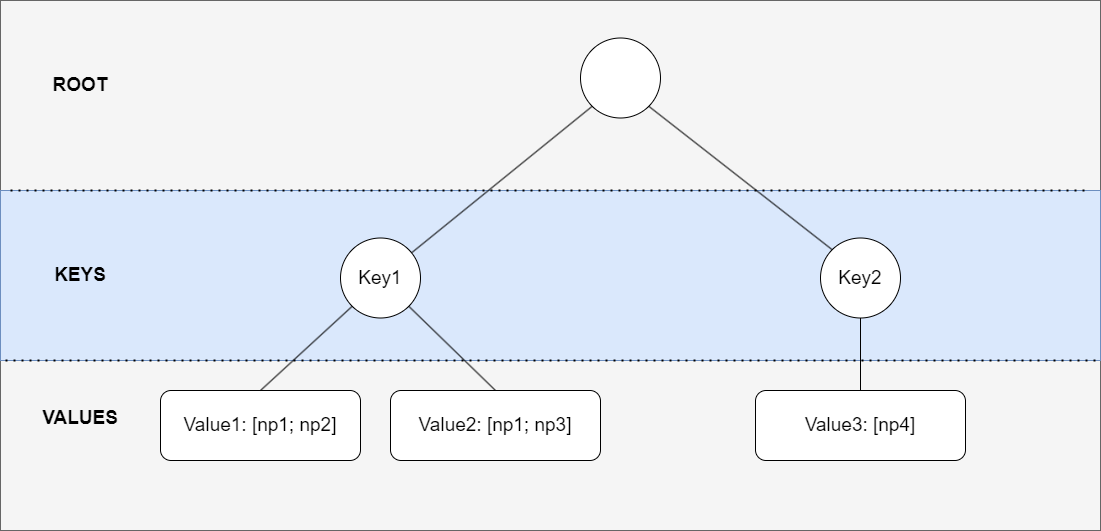
\includegraphics[width=0.8\textwidth]{images/labeltree.png}
  \caption{Structure of a Labeltree}
  \label{fig:labeltree}
\end{figure}

\newpage
% ==============================================
\section{Kubernetes Information Cluster} \label{impl:Kic}
The \acrshort{k8s} Information Cluster has two main functionalities: store all information about the current cluster state and update the cluster state given an event. To achieve this first functionality the \acrshort{kic} stores the following variables:
\begin{itemize}
    \renewcommand{\labelitemi}{\scriptsize$\blacksquare$}
    \item \textit{egressTree:} The egress tree is a Labeltree used to store all the egress policies in the current cluster state.
    \item \textit{ingressTree:} The ingress tree is a Labeltree used to store all the ingress policies in the current cluster state.
    \item \textit{reachabilitymatrix:} This is a ReachabilityMatrix data structure that stores the current state in the forn of a reachabilityMatrix and corresponding variables, as described in \autoref{impl:model}.
    \item \textit{pods:} A list of current containers
    \item \textit{pols:} A list of current network policies
\end{itemize}
Additionally, the \acrshort{kic} also offers functions to update these variables. 
\\[10pt]
For the second functionality of updating the current cluster state and reachabilitymatrix when given an event, different functions are required for different events. But before we can describe these functions we need to look at two smaller portions of the algorithm that reoccur often: getting all the containers that match all the label selectors in the allow set and similarly for the select set.
\\[10pt]

Both these algorithms use the same principle: for each label in a set of label selectors, we retrieve the bit array of containers that have this label applied according to the label\_map (see \autoref{kano:prefiltration}). We then do a bitwise AND operation to find the containers that have all these labels. When looking for the containers of the allow section of a \acrshort{np} we must take into account that multiple label selector sets can exist. Therefore we retrieve the containers for each set separately and use a bitwise OR operation to find the final containers. This is described in \autoref{algo:select} and \autoref{algo:allow}. 
\\[10pt]
\begin{algorithm}
    \caption{Find containers matching the select labelselectors of a given policy}
    \label{algo:select}
    \begin{algorithmic}[1]
    \State \textbf{Input:} a network policy
    \State \textbf{Output:} bitarray of containers matching the select labelselector
    \State 
    \State  select\_containers\_final $\gets$ bitarray(0 * amount of containers)
    \State first $\gets$ True

    \For{select\_label in policy.selector}
        \State containers $\gets$ new\_reach.label\_map.get(select\_label)
        \If{containers is not empty}
            \If{first}
                \State first $\gets$ False
                \State select\_containers $\gets$ containers
            \Else
                \State select\_containers AND containers
            \EndIf
        \Else:
            \State select\_containers $\gets$ bitarray(0 * amount of containers)
            \State break
        \EndIf
    \EndFor

  \end{algorithmic}
\end{algorithm}
\begin{algorithm} 
    \caption{Find containers matching the allow labelselectors of a given policy} 
    \label{algo:allow}
    \begin{algorithmic}[1]  
    \State \textbf{Input:} a network policy
    \State \textbf{Output:} bitarray of containers matching the allow labelselector
    \State 
    \State  allow\_containers\_final $\gets$ bitarray(0 * amount of containers)
    \For{allow in policy.allow}
        \State allow\_containers $\gets$ bitarray(0 * amount of containers)
        \State first $\gets$ True
        
        \For{allow\_label in allow}
           \State containers $\gets$ new\_reach.label\_map.get(allow\_label)
           \If{containers is not empty}
                \If{first}
                    \State first $\gets$ False
                    \State allow\_containers $\gets$ containers
                \Else
                    \State allow\_containers AND containers
                \EndIf
            \Else:
                \State allow\_containers $\gets$ bitarray(0 * amount of containers)
                \State break
            \EndIf
        \EndFor
        \State allow\_containers\_final OR allow\_containers
    \EndFor
  \end{algorithmic}
\end{algorithm}

\newpage
For the final part of this subsection, we will describe the functions in the \acrshort{kic} that are responsible for handling the events described in \autoref{tab:events} with the execption of update events. Since each update has differences regarding the values that changed within the object the function handling these events would have to take into account many variables. Simply calling the delete and create methods shortly after one another will get the same result instead. The functions that we created for the other four events all take an object as a parameter which is either a container or policy object as seen in \autoref{impl:model}. We will now briefly describe each function and show their implementation in pseudo-code.  
\\[10pt]
\begin{itemize}
    \item \textbf{Delete \acrshort{np} (\autoref{algo:deletepolicy}):} To delete a \acrshort{np} we first copy the existing reachabilitymatrix to the new reachabilitymatrix. We then use \autoref{algo:select} and \autoref{algo:allow} to get bit arrays of all the containers that respectively match the select and allow label selectors. We use the labels of each container in the allow\_containers bit array to find policies in the opposite direction with matching selector labels (i.e. if the deleted policy is ingress we look for an egress policy). In the following step, we only need to check if these opposite policies match the select\_containers of the deleted policy with their allow label selectors. If this is the case we have a match and need to remove the responsible policies for these 2 containers, as well as update the matrix to include a 0 at the correct position if no other responsible policies between these containers exist.
    
    \item \textbf{add \acrshort{np} (\autoref{algo:addpolicy}):} To add a \acrshort{np} we follow the same steps as in the delete policy algorithm: we find the select container, the allow containers and the opposite policies, and if they all align we have a match. However, we now add a 1 to the correct position in the reachabilitymatrix and add to the resp\_policies instead of removing from it.
    
    \item \textbf{Delete Container (\autoref{algo:deletecontainer}):} To delete a container we first create a new reachabilitymatrix with one less row and column than the existing current state reachabilitymatrix. We then iterate over all the existing containers, get their corresponding row in the existing reachabilitymatrix, and remove the bit that corresponds to the deleted container before adding the edited row to the new reachabilitymatrix. We update the matrix\_ids by decrementing each one that is higher than the removed container's matrix\_id. Updating the label\_map of the containers is done similarly as to how the matrix has been updated: going over each bit array, removing the bit corresponding to the removed container and moving each bit behind the removed bit up by 1 position. Lastly, the empty bit arrays get removed from the label\_map to remove unused labels.
    
    \item \textbf{Add Container (\autoref{algo:addcontainer}):} To add a container we first copy the existing reachabilitymatrix into the new\_reach variable and give a new matrix\_id to the container. By assigning a matrix\_id higher than that of all other containers we can guarantee that the new container is added at the end of the matrix for better visualization. Next, we add a 0 on the end of each existing bit array and append a row of zeroes to the end of the reachabilitymatrix. following this we find all rules that are applied to this new container and store them in the rules set which will be traversed to find the containers that match the allow selectors of these rules using \autoref{algo:allow}. Now that we have a container that is selected by a policy that selects our new container, we must only find another \acrshort{np} in the opposite direction. If such a \acrshort{np} exists a 1 is added on the correct position of the reachabilitymatrix and all the related variables are updated.
    
\end{itemize}

\begin{algorithm}
    \caption{Delete policy from reachability matrix}
    \label{algo:deletepolicy}
    \begin{algorithmic}[1]
        \Function{reachabilitydeleteNP}{policy}
            \State new\_reachability $\gets$ kic.reachabilitymatrix
            \State select\_containers $\gets$ \autoref{algo:select}
            \State allow\_containers $\gets$ \autoref{algo:allow} 
            \State opposite\_policies $\gets$ \{\}
            \For{allow\_container in allow\_containers where bit == 1}
                \For{label in allow\_container.labels}
                    \If{policy is ingress}
                        \State treenode = egressTree.find(label)
                    \Else
                        \State treenode = ingressTree.find(label)
                    \EndIf
                    \For{policy2 in treenode}
                        \If{all labels in policy2.selector are in allow\_container.labels}
                            \State  opposite\_policies.add((policy2, allow\_container))
                        \EndIf
                    \EndFor
                \EndFor
            \EndFor
            
            \For{(policy2, allow\_container) in opposite\_policies}
                \For{select\_container in select\_containers where bit == 1}
                    \For{allow in policy2.allow}
                        \If{all labels from allow in select\_container.labels}
                            \State remove policy and policy2 from resp\_policies for the containers
                            \If{no responsible policies between the containers exist}
                                \State set bit in reachabilitymatrix to 0
                            \EndIf
                        \EndIf
                    \EndFor
                \EndFor
            \EndFor
            \State update variables
            \State \textbf{return} (new\_reachability)
        \EndFunction
  \end{algorithmic}
\end{algorithm}

\begin{algorithm}
    \caption{add policy to reachability matrix}
    \label{algo:addpolicy}
    \begin{algorithmic}[1]
        \Function{reachabilityaddNP}{policy}
            \State new\_reachability $\gets$ kic.reachabilitymatrix
            \State select\_containers $\gets$ \autoref{algo:select}
            \State allow\_containers $\gets$ \autoref{algo:allow} 
            \State opposite\_policies $\gets$ \{\}
            \For{allow\_container in allow\_containers where bit == 1}
                \For{label in allow\_container.labels}
                    \If{policy is ingress}
                        \State treenode = egressTree.find(label)
                    \Else
                        \State treenode = ingressTree.find(label)
                    \EndIf
                    \For{policy2 in treenode}
                        \If{all labels in policy2.selector are in allow\_container.labels}
                            \State  opposite\_policies.add((policy2, allow\_container))
                        \EndIf
                    \EndFor
                \EndFor
            \EndFor
            
            \For{(policy2, allow\_container) in opposite\_policies}
                \For{select\_container in select\_containers where bit == 1}
                    \For{allow in policy2.allow}
                        \If{all labels from allow in select\_container.labels}
                            \State add policy and policy2 to resp\_policies for the containers
                            \State set bit in reachabilitymatrix to 1
                        \EndIf
                    \EndFor
                \EndFor
            \EndFor
            \State update variables
            \State \textbf{return} (new\_reachability)
        \EndFunction
  \end{algorithmic}
\end{algorithm}

\begin{algorithm}
    \caption{Delete container from reachability matrix}
    \label{algo:deletecontainer}
    \begin{algorithmic}[1]
        \Function{reachabilityDeleteContainer}{container}
            \State new\_reachability $\gets$ $nXn$ matrix of bitarrays of 0's, with  n = \# of containers
            \State \Comment{Updating the reachability matrix}
            \For{i, cont in enumerate(containers)}
                \State row $\gets$ reachabilitymatrix[cont.matrix\_id]
                \State row.pop(cont.matrix\_id) \Comment{bit for the removed container}
                
                \If{container.matrix\_id \texttt{>} container.id}
                    \State container.matrix\_id -= 1
                \EndIf
                \State store row in new\_reachability
            \EndFor
            
            \State \Comment{Updating the label\_map matrix}
            \State new\_label\_map $\gets$ \{\}
            \For{label, old\_arr in reachabilitymatrix.label\_map.items()}
                \For{k in range(len(old\_arr))}
                    \If{k \texttt{>} container.matrix\_id}
                       \State new\_label\_map[label][k - 1] $\gets$ old\_arr[k] 
                    \ElsIf{k \texttt{<} container.matrix\_id}
                        \State new\_label\_map[label][k] $\gets$ old\_arr[k] 
                    \EndIf
                \EndFor
            \EndFor

            \State \Comment{Removing empty bitarrays from label\_map}
            \State new\_label\_map\_v2 $\gets$ \{\}
            \For{label, arr in new\_label\_map.items()}
                \If{\textbf{not} any bits set in arr}
                    \State delete new\_label\_map\_v2[label]
                \EndIf
            \EndFor
        
            \State new\_reachability.label\_map $\gets$ new\_label\_map\_v2
        
            \For{pod in pods}
                \If{pod.matrix\_id \texttt{>} container.matrix\_id}
                    \State pod.matrix\_id -= 1
                \EndIf
            \EndFor
        
            \State \textbf{return} (new\_reachability)
        \EndFunction
  \end{algorithmic}
\end{algorithm}

\begin{algorithm}
    \caption{Add container to reachability matrix}
    \label{algo:addcontainer}
    \begin{algorithmic}[1]
    \Function{reachabilityAddContainer}{container}
        \State new\_reach $\gets$ kic.reachabilitymatrix
        \State container.matrix\_id $\gets$ len(containers)
        \State matrixId\_to\_Container[container.matrix\_id] = container
        \For{label, array in label\_map}
            \State array.append(False)
        \EndFor
        \For{row in new\_reach} 
            \State row.append(0)
        \EndFor
        \State new\_reach.append(bitarray(0 * amount of containers))
        \State rules = Set()
        \For{label in container.labels}: 
            \For{policy in eggressTrie.find(label)}
                \If{all policy.select.label in container.labels}
                    \State rules.add
                \EndIf
            \EndFor
            \For{policy in ingressTrie.find(label)}
                \If{all policy.select.label in container.labels}
                    \State rules.add
                \EndIf
            \EndFor
        \EndFor
        \For{rule in rules}
            \State allow\_containers $\gets$ \autoref{algo:allow} 
            \For{secondcontainer in allow\_containers}
                secondRules = Set()
                \For{secondlabel in secondcontainer.labels}:
                    \For{policy in eggressTrie.find(label)}
                        \If{all policy.select.label in container.labels}
                            \State secondRules.add
                        \EndIf
                    \EndFor
                    \For{policy in ingressTrie.find(label)}
                        \If{all policy.select.label in container.labels}
                            \State secondRules.add
                        \EndIf
                    \EndFor
                \EndFor
                \For{secondrule in secondRules}
                    \If{all labels of secondrule.selector in secondcontainer}
                        \For{secondallow in secondrule.allow}
                            \If{all labels of secondallow in container.labels}
                                \State update the matrix for new connection
                            \EndIf
                        \EndFor
                    \EndIf
                \EndFor    
            \EndFor 
        \EndFor   
        \State \textbf{return} new\_reachability
    \EndFunction
  \end{algorithmic}
\end{algorithm}



% ==============================================
\newpage
\section{Security Group Information Cluster} \label{impl:sgic}
Since handling cloud layer events is out of scope for this thesis we also do not need to actively monitor the cloud layer. Therefore the \acrlong{sgic} mimics the security groups and security group rules one might find in the cloud layer by generating them with randomised variables when the Watcher is initialized. Security group objects are based upon the OpenStack Security Group definitions, which means they contain a list of rules and have a unique name \cite{secgroups}. The amount of rules in each security group is randomised as well, and each rule contains variables such as port, direction, protocol and ethertype filled with randomised values. Additionally, a security group rule targets other nodes by either a single remote IP, an IP with a subnetmask to act as a range of IPs, or the name of another existing security group which targets all nodes part of that security group.
\\[10pt]

Once the security groups and their rules are created each node in the \acrshort{k8s} cluster gets linked to one or multiple security groups. We then use directed graphs to store allowed connections, where nodes are the vertices and an edge between two nodes indicates that connection is allowed in that direction. Each edge includes the security group and security group rule number responsible for the connection. Thereafter both an ingress and egress graph get created and filled by going through all security groups, finding their nodes and adding the corresponding security group rules to these nodes in the graphs. We then use these 2 directed graphs to create a VMmatrix of size \(kxk\) where \(k\ =\ amount\  of\  nodes\  in\  the\  cluster\), similarly to the Kano reachabilitymatrix. When an edge is present in both graphs the connection is allowed in both directions and thus results in a 1 in the VMmatrix. Since we created the directed graphs we can easily retrieve responsible security groups and security group rules for a specific node connection. The VMmatrix on the other hand quickly tells us whether or not the connection is possible in the first place.
\\[10pt]

The \acrlong{sgic} is also responsible for conflict detection between the cloud and cluster layer. Once the \acrshort{kic} finishes creating the updated reachabilitymatrix the Analyzer will call the check\_sg\_connectivity function in the \acrshort{sgic} which we will now explain with the help of \autoref{algo:connectivity}. The function takes three parameters: 2 node names and a boolean indicating whether or not a connection between these 2 nodes is wanted. E.g. a newly created container can communicate with another container on a different node: then the function gets called with the boolean connection\_wanted set to True. The function will then print out whether or not the nodes can communicate by looking at the VMmatrix and print out the responsible security groups and security group rules by retrieving them from the directed graphs. If the connection is contradictory to the boolean we report a conflict.

\begin{algorithm}
    \caption{Conflict detection}
    \label{algo:connectivity}
    \begin{algorithmic}[1]
    \Function{check\_sg\_connectivity}{node1, node2, connection\_wanted}
        \State print security groups for node1
        \State print security groups for node2
        \If{vmMatrix[node1, node2] == 1}
            \If{connection\_wanted == True}
                \State print security group rules responsible for connection 
            \Else
                \State report conflict with responsible security group rules
            \EndIf
        \EndIf
        \If{vmMatrix[node2, node1] == 1}
            \If{connection\_wanted == True}
                \State print security group rules responsible for connection 
            \Else
                \State report conflict with responsible security group rules
            \EndIf
        \EndIf
    \EndFunction
  \end{algorithmic}
\end{algorithm}





\cleardoublepage


